\documentclass[11pt,a4paper]{article}

% Typeface: XeLaTeX with Latin Modern Roman (fontspec default)
\usepackage{fontspec}
\usepackage{polyglossia}
\setdefaultlanguage{turkish}

% Page: the measures of the note template (A4, 11 pt, 4.5 cm side margins, header and page count)
\usepackage[a4paper,left=4.5cm,right=4.5cm,top=4.5cm,bottom=4.1cm,headheight=14pt,headsep=0.55cm,
  footskip=0.55cm]{geometry}
\linespread{0.946}
\usepackage{fancyhdr}
\usepackage{lastpage}
\pagestyle{fancy}
\fancyhf{}
\fancyhead[L]{\small\textbf{PROJE NOTU} $|$ Coin flipping}
\fancyhead[R]{\small\textbf{Derlenme tarihi:} \today}
\fancyfoot[C]{\small\thepage\,/\,\pageref{LastPage}}
\renewcommand{\headrulewidth}{0.4pt}

\usepackage{microtype}
\usepackage{amsmath,amssymb}
\usepackage{booktabs,array,tabularx}
\usepackage{graphicx}
\usepackage{enumitem}
\setlist{noitemsep, topsep=3pt, leftmargin=*}
\usepackage{xcolor}
\definecolor{secblue}{HTML}{1F3A5F}
\definecolor{boxback}{HTML}{EEF2F6}
\definecolor{mark}{HTML}{9B2226}
\definecolor{hl}{HTML}{FFF36B}
\usepackage{titlesec}
\titleformat{\section}{\color{secblue}\bfseries\normalsize}{\thesection.}{0.4em}{}
\titlespacing*{\section}{0pt}{10pt}{4pt}
\usepackage[font=small,labelfont=bf,labelsep=period,skip=4pt]{caption}
\usepackage[bottom]{footmisc}
\captionsetup[figure]{name=Şekil}
\captionsetup[table]{name=Tablo}
\setlength{\parindent}{0pt}
\setlength{\parskip}{5pt}
\setlength{\textfloatsep}{10pt}
\emergencystretch=3em

\newcommand{\Paths}{2.000}
\newcommand{\ShareNow}{5{,}1}
\newcommand{\ShareByThousand}{53{,}1}
\newcommand{\ShareByMax}{74{,}4}
\newcommand{\ShareByMaxSe}{1{,}0}
\newcommand{\RmsSlope}{-0{,}496}
\newcommand{\RmsOverSe}{1{,}009}
\newcommand{\LilFrom}{922}
\newcommand{\LilThreeSigma}{1{,}2\times 10^{39}}
\newcommand{\NBelowHalf}{1.904}
\newcommand{\SlopeHalf}{-0{,}500}
\newcommand{\NBelowTenth}{7.129}
\newcommand{\SlopeTenth}{-0{,}500}
\newcommand{\NBelowHundredth}{80.246}
\newcommand{\SlopeHundredth}{-0{,}499}
\newcommand{\DHalfThirty}{0{,}072}
\newcommand{\DccHalfThirty}{$9{,}2\times 10^{-4}$}
\newcommand{\DHalfThousand}{0{,}0126}
\newcommand{\DccHalfThousand}{$2{,}7\times 10^{-5}$}
\newcommand{\DccHalfTenThousand}{$2{,}7\times 10^{-6}$}
\newcommand{\DccRatioHalf}{10{,}0}
\newcommand{\DccRatioTenth}{3{,}16}
\newcommand{\DRootNHalf}{0{,}3989}
\newcommand{\DHundredthThirty}{0{,}45}
\newcommand{\BeOverDHalf}{1{,}19}
\newcommand{\BeOverDHundredth}{1{,}78}
\newcommand{\HistN}{30}
\newcommand{\HistM}{20.000}
\newcommand{\VoneBins}{72}
\newcommand{\VoneWidth}{0{,}0097}
\newcommand{\Spacing}{0{,}0333}
\newcommand{\VoneEmpty}{51}
\newcommand{\VoneMax}{15{,}3}
\newcommand{\LatticeMax}{4{,}45}
\newcommand{\ExactMax}{4{,}33}
\newcommand{\NormalPeak}{4{,}37}
\newcommand{\PeakRatio}{3{,}5}


\begin{document}


\vspace*{14pt}
\begin{tabular}{@{}p{2.35cm}@{}p{\dimexpr\textwidth-2.35cm}@{}}
\textbf{BAŞLIK:} & \textbf{\large Yazı tura: yürüyen ortalama, \%95 bandı ve normal yaklaşım gerçekte neyi gösterir}\\[3pt]
\textbf{KONU:} & \texttt{coin-flipping-exercise} deposunun 2.\ sürümündeki analizlerin amacı, yöntemi ve sonuçları\\[3pt]
\textbf{YAZAR:} & Muhammed İkbal Yılmaz (myucanlar@gmail.com)
\end{tabular}

\vspace{8pt}
\vspace{12pt}

\section{Amaç ve kapsam}

$X_1, X_2, \dots$ bir madeni paranın bağımsız atışları olsun; $p$ olasılıkla $X_i = 1$ (yazı) gelsin ve
$\hat p_n = \frac1n\sum_{i=1}^n X_i$, $n$ atış sonundaki yazı oranı olsun. Bu oranın standart hatası
$\mathrm{SH}(n) = \sqrt{p(1-p)/n}$'dir. Projenin 1.\ sürümü iki klasik sonucu benzetimle göstermişti: büyük sayılar yasasını
(BSY), $p \pm 1{,}96\,\mathrm{SH}(n)$ bandı içinde çizilen bir yürüyen ortalama $\hat p_n$ ile; merkezî limit teoremini (MLT)
ise çok sayıda tekrarlanan deneydeki $\hat p_n$ değerlerinin histogramı ve üzerine çizilen normal eğri ile. Her iki gösterim de
göz kararıyla değerlendirilmişti. Bu not, her görsel izlenimin yerine ölçülen ya da kesin olarak hesaplanan bir büyüklük
koyar ve üç soru sorar:

\begin{enumerate}
  \item \textbf{Yürüyen ortalamanın etrafındaki \%95 bandı ne söyler?} Özellikle, tek bir yol bu bandın içinde kalmalı mıdır?
  \item \textbf{Normal yaklaşım kaç atışa ihtiyaç duyar,} ve bu sayı $p$'ye ve süreklilik düzeltmesine nasıl bağlıdır? 1.\
  sürümdeki hilesiz para ($p = 0{,}5$) en elverişli durumdur; $p = 0{,}1$ ve $p = 0{,}01$, uygulamada sık karşılaşılan küçük
  oranları (nadir olaylar, düşük yanıt oranları) temsil eder.
  \item \textbf{1.\ sürümün histogramları neden sivri çıkıntılı görünüyordu,} ve bir örnek oranı nasıl sınıflara ayrılmalıdır?
\end{enumerate}

\section{Yöntem}

\begin{itemize}
  \item \textbf{Benzetim.} Sabit tohumlu NumPy varsayılan üreteci. Yürüyen ortalamalar tamsayı yazı sayılarından hesaplanır,
  dolayısıyla kesin oranlardır. $n$ atışlık her tekrar deneyi doğrudan bir binom sayısı olarak çekilir.
  \item \textbf{Kesin hesaplar.} $S_n \sim \mathrm{Bin}(n,p)$ binom dağılımı logaritmik ölçekte hesaplanır. Binom ile normal
  dağılım arasındaki uzaklık Kolmogorov uzaklığıdır: $D_n = \sup_x \lvert P(S_n \le x) - \Phi\bigl((x-np)/\sigma_n\bigr)\rvert$,
  $\sigma_n = \sqrt{np(1-p)}$. Binom dağılım fonksiyonu basamak fonksiyonu olduğundan supremum sıçramalarından birinde
  gerçekleşir; bu yüzden $D_n$, her sıçramanın iki yanı denetlenerek kesin olarak hesaplanır. Süreklilik düzeltmesinde
  $P(S_n \le k)$, $\Phi\bigl((k+0{,}5-np)/\sigma_n\bigr)$ ile yaklaşıklanır.
  \item \textbf{Sınırlar.} Berry--Esseen eşitsizliği $D_n \le C\rho/(\sigma^3\sqrt n)$ verir; tek atış için $\sigma^2 = pq$ ve
  $\rho = E|X-p|^3 = pq(p^2+q^2)$, $q = 1-p$'dir. Yayımlanmış en iyi sabit $C < 0{,}4748$ kullanılmıştır (Shevtsova, 2011).
  Yinelenmiş logaritma yasası (YLY; yazı tura için Khintchine, 1924; Hartman ve Wintner, 1941), olasılık bir ile
  $\limsup_n \lvert\hat p_n - p\rvert / \sqrt{2p(1-p)\log\log n/n} = 1$ olduğunu söyler.
  \item \textbf{Denetimler.} On birim testi kodu bağımsız hesaplarla karşılaştırır: binom olasılıklarını kesin rasyonel
  aritmetikle, $D_n$'yi ince bir ızgara üzerinde kaba kuvvet aramasıyla, yürüyen ortalamaları düz bir döngüyle.
\end{itemize}

\section{Analiz 1: Yürüyen ortalama ve noktasal bant (Şekil~\ref{fig:lln})}

\textbf{Neden.} 1.\ sürüm tek bir yürüyen ortalamayı $p \pm 1{,}96\,\mathrm{SH}(n)$ bandı içinde çizmiş, bunu \%95 bandı olarak
adlandırmış ve yolun $p$'ye yakın kaldığını belirtmişti. Bant noktasaldır: her sabit $n$ için $\hat p_n$ yaklaşık \%95
olasılıkla bandın içindedir. Ancak bütün bir yola bakan okuyucu bandı, doğal olarak, yolun içinde kalması gereken bir bölge
gibi okur. Bunlar farklı önermelerdir; bu analiz ikisini de ölçer.

\textbf{Yöntem.} $10^5$ hilesiz para atışından oluşan \Paths{} bağımsız yol. Her $n$ için: $n$'de bandın dışında olan yolların
payı; $n$'ye kadar en az bir kez dışarı çıkmış yolların payı; ve $\hat p_n - p$'nin karesel ortalamasının karekökü (KOK).

\textbf{Şekil nasıl okunmalı.} Solda: yollardan 20'si, bant (siyah) ve YLY zarfı (gri, kesikli). Sağda: mavi eğri belirli bir
$n$'de dışarıda olanların payıdır ve bant doğruysa kırmızı noktalı \%5 çizgisine yakın olmalıdır; siyah eğri bir noktada banttan
çıkmış olanların payıdır.

\begin{figure}[h]
\centering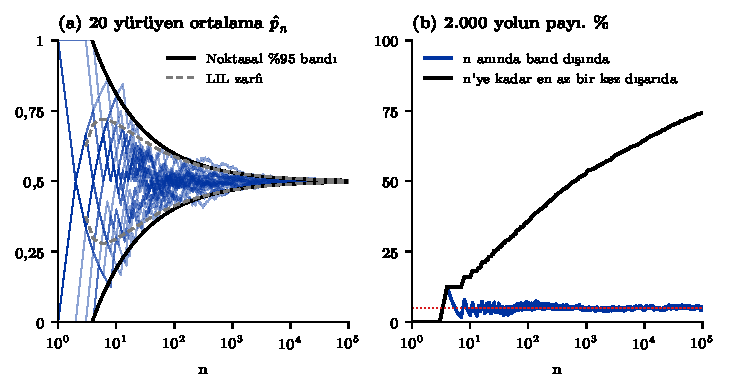
\includegraphics[width=\textwidth]{../figures/tr/fig1_lln.pdf}
\caption{Solda: 20 hilesiz para yolunun yürüyen ortalamaları, noktasal \%95 bandı ve YLY zarfı. Sağda: \Paths{} yoldan $n$'de
bandın dışında olanların ve $n$'ye kadar en az bir kez dışarı çıkmış olanların payı. Noktalı: \%5.}\label{fig:lln}
\end{figure}

\textbf{Bulgu.} Bant noktasal olarak doğrudur: $10^3 \le n \le 10^5$ için belirli bir $n$'de yolların ortalama
\%\ShareNow'i bandın dışındadır. Ancak yolların \%\ShareByThousand'i $n = 10^3$'e, \%\ShareByMax'ü $n = 10^5$'e kadar en az bir
kez banttan çıkmıştır (Monte Carlo standart hatası \ShareByMaxSe{} yüzde puan) ve eğri hâlâ yükselmektedir. YLY'nin öngördüğü
budur: zarf her $n \ge \LilFrom$ için banttan geniştir ($\sqrt{2\log\log n} > 1{,}96$ olduğu yerde), dolayısıyla olasılık bir
ile her yol banttan sonsuz kez çıkar ve siyah eğri \%100'e yaklaşır. Aynısı $3\sigma$ bandı için de geçerlidir, ancak orada
zarfın bandı aştığı nokta yaklaşık $\LilThreeSigma$ atıştır, yani herhangi bir benzetimin çok ötesindedir. KOK hata log--log
ölçekte $\RmsSlope$ eğimiyle azalır ve $n = 10^5$'te $\RmsOverSe\,\mathrm{SH}(n)$'ye eşittir: BSY'nin $1/\sqrt n$ hızı tam
öngörüldüğü gibi gerçekleşir.

\textbf{Yorum.} Bant ``bu $n$ için $\hat p_n$ büyük olasılıkla nerededir?'' sorusunu yanıtlar; ``yol nerede kalacak?'' sorusunu
değil. Banttan çıkan bir yol $p = 0{,}5$ aleyhine kanıt değildir. 1.\ sürümün ``$n \approx 10^4$'te yürüyen ortalama 0,5'e çok
yakındır'' ifadesi kesinleştirilebilir: $n = 10^4$'te $\mathrm{SH} = 0{,}005$'tir, yani $\hat p_n$ o $n$'de \%95 olasılıkla
$p$'nin $\pm 0{,}0098$ yakınındadır. Tüm $n$'ler için aynı anda geçerli bir bant, büyük $n$'lerde YLY zarfından geniş olmak
zorundadır.

\section{Analiz 2: Normal yaklaşımın doğruluğu (Şekil~\ref{fig:clt}, Tablo~\ref{tab:clt})}

\textbf{Neden.} 1.\ sürüm MLT'yi benzetilmiş histogramlardan değerlendirmişti; bu, yaklaşım hatasını benzetim gürültüsü ve sınıf
seçimiyle (bkz.\ analiz 3) karıştırır. Binom dağılımı ile normal yaklaşımı arasındaki uzaklık kesin olarak hesaplanabilir ve
Berry--Esseen sınırı bu uzaklığın ne kadar büyük olabileceğini söyler. Yaygın bir pratik kural $n \ge 30$'un yeterli olduğunu
söyler; soru, ulaşılan doğruluğun $p$'ye bağlı olup olmadığıdır.

\textbf{Yöntem.} $p \in \{0{,}5;\ 0{,}1;\ 0{,}01\}$ ve 5 ile $10^5$ arasında logaritmik ölçekte eşit aralıklı 46 $n$ değeri için:
süreklilik düzeltmeli ve düzeltmesiz $D_n$ ile Berry--Esseen sınırı.

\textbf{Şekil nasıl okunmalı.} İki eksen de logaritmiktir; $n^{-1/2}$ ile orantılı bir büyüklük $-1/2$ eğimli bir doğrudur. Düz
çizgiler kesin uzaklıklar, kesikli çizgiler aynı renkteki sınırlardır; noktalı çizgi $D_n = 0{,}01$ düzeyini gösterir.

\begin{figure}[h]
\centering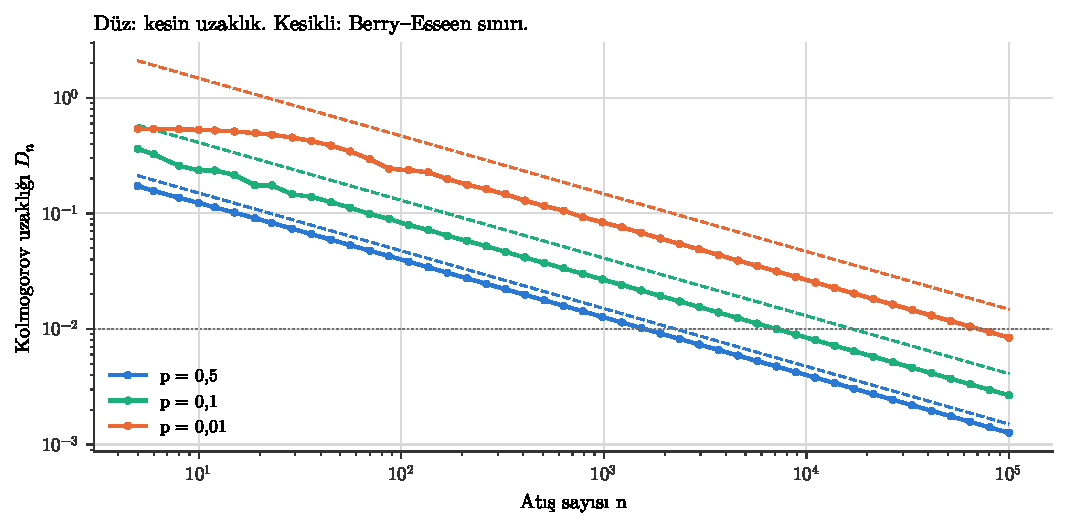
\includegraphics[width=\textwidth]{../figures/tr/fig2_clt_accuracy.pdf}
\caption{$\mathrm{Bin}(n,p)$ ile normal yaklaşımı arasındaki kesin Kolmogorov uzaklığı (düz) ve $C = 0{,}4748$ ile
Berry--Esseen sınırı (kesikli). Noktalı: $0{,}01$.}\label{fig:clt}
\end{figure}

\begin{table}[h]
\centering\footnotesize
\caption{Süreklilik düzeltmesiz ve düzeltmeli (sd) kesin Kolmogorov uzaklığı $D_n$ ve 46 $n$ değeri arasında $D_n$'nin
$0{,}01$'in altında kaldığı ilk değer.}\label{tab:clt}
\scriptsize\setlength{\tabcolsep}{1.7pt}
\begin{tabular}{@{}lrrrrrrrrr@{}}
\toprule
 & \multicolumn{2}{c}{$n = 30$} & \multicolumn{2}{c}{$n = 100$} & \multicolumn{2}{c}{$n = 1000$} & \multicolumn{2}{c}{$n = 10^4$} & $D_n < 0{,}01$ \\
\cmidrule(lr){2-3}\cmidrule(lr){4-5}\cmidrule(lr){6-7}\cmidrule(lr){8-9}
$p$ & $D_n$ & sd & $D_n$ & sd & $D_n$ & sd & $D_n$ & sd & için $n$ \\
\midrule
$0{,}5$ & 0{,}0722 & $9{,}2\times 10^{-4}$ & 0{,}0398 & $2{,}7\times 10^{-4}$ & 0{,}0126 & $2{,}7\times 10^{-5}$ & 0{,}00399 & $2{,}7\times 10^{-6}$ & 1.904 \\
$0{,}1$ & 0{,}147 & 0{,}0309 & 0{,}0832 & 0{,}0175 & 0{,}0266 & 0{,}00560 & 0{,}00842 & 0{,}00177 & 7.129 \\
$0{,}01$ & 0{,}449 & 0{,}0965 & 0{,}236 & 0{,}0584 & 0{,}0830 & 0{,}0204 & 0{,}0266 & 0{,}00654 & 80.246 \\
\bottomrule

\end{tabular}
\end{table}

\textbf{Bulgu.} Her $p$ için uzaklık $n^{-1/2}$ gibi azalır ($n \ge 10^3$ için eğimler $\SlopeHalf$, $\SlopeTenth$,
$\SlopeHundredth$); bu, Berry--Esseen eşitsizliğinin izin verdiği hızdır ve sınır gevşek değildir: $n = 1000$'de sınır,
$p = 0{,}5$ için kesin uzaklığın \BeOverDHalf{}, $p = 0{,}01$ için \BeOverDHundredth{} katıdır. Hilesiz para için $n = 10^4$'te
$\sqrt n\,D_n = \DRootNHalf$'dur; bu $1/\sqrt{2\pi} \approx 0{,}3989$'a eşittir: hata, sürekli bir eğrinin izleyemeyeceği
binom dağılım fonksiyonunun en büyük sıçramasının yarısıdır. Gereken atış sayısı büyük ölçüde $p$'ye bağlıdır: $D_n$,
$p = 0{,}5$ için $n = \NBelowHalf$'ten, $p = 0{,}1$ için $n = \NBelowTenth$'dan, $p = 0{,}01$ için $n = \NBelowHundredth$'dan
itibaren $0{,}01$'in altında kalır (ızgaradaki ilk değerler). $n = 30$'da uzaklık $p = 0{,}5$ için \DHalfThirty{}, $p = 0{,}01$
için ise \DHundredthThirty{}'tir. Süreklilik düzeltmesi sıçrama hatasını giderir: $p = 0{,}5$ için $D_{30}$ değerini \DccHalfThirty{}
düzeyine indirir ve $n = 1000$'den $10^4$'e düzeltilmiş uzaklık \DccRatioHalf{} kat, yani $1/n$ gibi azalır. $p = 0{,}1$ için düzeltilmiş
uzaklık yalnızca \DccRatioTenth{} $\approx \sqrt{10}$ kat azalır: geriye kalan hata, binom dağılımının çarpıklığından,
$(q-p)/\sqrt{npq}$, kaynaklanır; bu çarpıklık yalnızca $p = 0{,}5$'te sıfırdır ve simetrik bir normal eğrinin hiçbir düzeltmesi
onu gideremez.

\textbf{Yorum.} ``$n \ge 30$'' MLT'nin bir özelliği değildir. Yaklaşımın ne kadar iyi olduğu, çarpıklık üzerinden $p$'ye ve
gereken doğruluğa bağlıdır. Hilesiz para için süreklilik düzeltmesi yaklaşımı daha $n = 30$'da çok isabetli kılar; küçük
oranlar için kesin binom olasılıkları daha güvenli seçimdir.

\section{Analiz 3: Bir örnek oranının histogramı (Şekil~\ref{fig:hist})}

\textbf{Neden.} 1.\ sürüm benzetilmiş oranları, 25--160 sınıfla sınırlandırılmış Freedman--Diaconis kuralıyla sınıflara ayırmıştı.
Küçük $n$'lerde bu kural normal eğrinin çok üzerinde, uzun ve dar çıkıntılar üretir (Şekil~\ref{fig:hist}, sol panel); bu
MLT'nin başarısızlığı gibi okunabilir. Oysa $\hat p_n$ kesiklidir: yalnızca $n+1$ tane $k/n$ değerini alır.

\textbf{Yöntem.} $n = \HistN$ hilesiz para atışından oluşan \HistM{} deney (1.\ sürümün $n = 30$ için kullandığı ayar) iki kez sınıflandırılır: 1.\ sürümün kuralıyla
(değiştirilmeden) ve $k/n$ değerlerine ortalanmış $1/n$ genişliğinde sınıflarla. Sağ panele kesin olasılıklar
$P(\hat p_n = k/n)$ eklenmiştir; histogramın yoğunluk ölçeğine taşımak için $n$ ile çarpılmışlardır.

\textbf{Şekil nasıl okunmalı.} İki panel de yoğunluk gösterir; her birinde çubukların toplam alanı 1'dir. Dikey eksen ortaktır
ve siyah eğri iki panelde de aynı normal yoğunluktur.

\begin{figure}[h]
\centering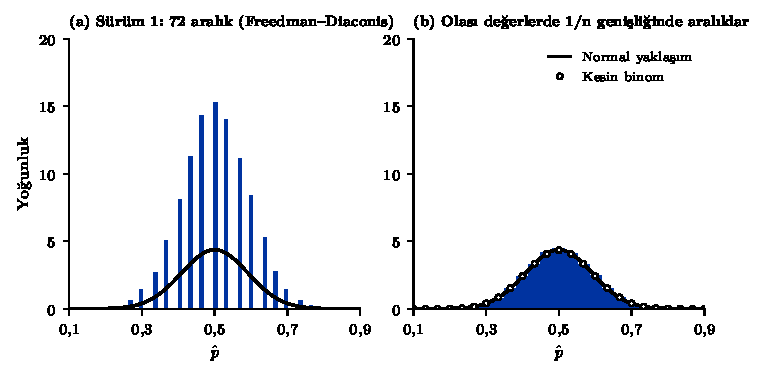
\includegraphics[width=\textwidth]{../figures/tr/fig3_histogram.pdf}
\caption{$n = \HistN$ atışlık \HistM{} örnek oranı. Solda: 1.\ sürümün sınıfları. Sağda: her olası değer için $1/n$ genişliğinde
bir sınıf ve kesin binom olasılıkları. Siyah: ortalaması $0{,}5$, varyansı $0{,}25/n$ olan normal yoğunluk.}\label{fig:hist}
\end{figure}

\textbf{Bulgu.} $\hat p_{30}$'un değerleri arasında $1/30 = \Spacing$ aralık vardır, ancak Freedman--Diaconis kuralı
\VoneWidth{} genişliğinde \VoneBins{} sınıf verir. Bu nedenle her olası değer tek bir dar sınıfa düşer ve değerler arasındaki
sınıflar boş kalır (\VoneBins{} sınıftan \VoneEmpty{} tanesi). Her çubuk aralığın yaklaşık üçte biri genişliğinde olduğundan
yüksekliği yaklaşık üç kat fazladır: en yüksek çubuk \VoneMax{}'e ulaşır, bu normal yoğunluğun tepe değeri olan
\NormalPeak{}'nin \PeakRatio{} katıdır. $1/n$ genişliğindeki sınıflarla en yüksek çubuk \LatticeMax{}'tir; kesin olasılık
\ExactMax{}, normal yoğunluk \NormalPeak{}'dir.

\textbf{Yorum.} Çıkıntılar MLT'nin başarısızlığı değil, sınıflandırmanın yarattığı bir yapaylıktı. Freedman--Diaconis kuralı
sürekli bir yoğunluktan gelen örnekler için türetilmiştir (Freedman ve Diaconis, 1981); kesikli verilerde sınıf genişliği olası
değerler arasındaki aralığın katı olmalıdır.

\section{Sonuçlar ve sınırlılıklar}

\begin{itemize}
  \item Noktasal \%95 bandı her $n$'de doğrudur, ama bir yolun içinde kaldığı bir bölge değildir: yolların dörtte üçü
  $n = 10^5$'e kadar banttan çıkmıştı ve YLY'ye göre her yol banttan sonsuz kez çıkar.
  \item Bir oranın normal yaklaşımı $n^{-1/2}$ gibi iyileşir ve gereken atış sayısı $p$'ye bağlıdır: $p$, $0{,}5$'ten $0{,}01$'e
  giderken $D_n < 0{,}01$ için yaklaşık $2.000$'den $80.000$'e çıkar. Süreklilik düzeltmesi $p = 0{,}5$ için hatanın büyük
  kısmını giderir, çarpık durumlarda çok daha azını.
  \item Kesikli verilerin histogramı olası değerlere uygun sınıflar gerektirir; aksi hâlde histogramın şekli MLT hakkında bir şey
  söylemez.
  \item Yalnızca bağımsız atışlar ve üç $p$ değeri incelenmiştir. Kolmogorov uzaklığı bir olasılıktaki en büyük hatayı ölçer;
  kuyruklardaki göreli hatayı ölçmez, bu çok daha büyük olabilir. $D_n < 0{,}01$ eşikleri 46 $n$ değerinden oluşan bir
  ızgara üzerinde verilmiştir. Analiz 1, $10^5$ uzunluğunda \Paths{} yol kullanır.
\end{itemize}

\section*{Kaynaklar}
{\small
\setlength{\parskip}{2pt}
\hangindent=1.27cm\hangafter=1 Freedman, D., \& Diaconis, P. (1981). On the histogram as a density estimator: $L_2$ theory. \textit{Zeitschrift für
Wahrscheinlichkeitstheorie und verwandte Gebiete}, 57(4), 453--476.\par
\hangindent=1.27cm\hangafter=1 Hartman, P., \& Wintner, A. (1941). On the law of the iterated logarithm. \textit{American Journal of Mathematics}, 63(1), 169--176.\par
\hangindent=1.27cm\hangafter=1 Khintchine, A. (1924). Über einen Satz der Wahrscheinlichkeitsrechnung. \textit{Fundamenta Mathematicae}, 6, 9--20.\par
\hangindent=1.27cm\hangafter=1 Shevtsova, I. G. (2011). On the absolute constants in the Berry--Esseen type inequalities for identically distributed summands.
arXiv:1111.6554.\par
\hangindent=1.27cm\hangafter=1 NumPy belgeleri: \texttt{numpy.random.Generator}.\par

\smallskip
Tüm sayılar
\texttt{figures/*.csv} dosyalarından \texttt{make\_paper.py} ile üretilmiştir.
}

\end{document}
